%\iffalse
\let\negmedspace\undefined
\let\negthickspace\undefined
\documentclass[journal,12pt,onecolumn]{IEEEtran}
\usepackage{cite}
\usepackage{amsmath,amssymb,amsfonts,amsthm}
\usepackage{algorithmic}
\usepackage{graphicx}
\usepackage{textcomp}
\usepackage{xcolor}
\usepackage{txfonts}
\usepackage{listings}
\usepackage{enumitem}
\usepackage{mathtools}
\usepackage{gensymb}
\usepackage{comment}
\usepackage[breaklinks=true]{hyperref}
\usepackage{tkz-euclide} 
\usepackage{listings}
\usepackage{gvv}    
\usepackage{enumitem}
\usepackage{amsmath}
\def\inputGnumericTable{}                                 
\usepackage[latin1]{inputenc}                                
\usepackage{color}                                            
\usepackage{array}                                            
\usepackage{longtable}                                       
\usepackage{calc}                                             
\usepackage{multirow}                                         
\usepackage{hhline}                                           
\usepackage{ifthen}                                           
\usepackage{lscape}
\usepackage{tabularx}

\newtheorem{theorem}{Theorem}[section]
\newtheorem{problem}{Problem}
\newtheorem{proposition}{Proposition}[section]
\newtheorem{lemma}{Lemma}[section]
\newtheorem{corollary}[theorem]{Corollary}
\newtheorem{example}{Example}[section]
\newtheorem{definition}[problem]{Definition}
\newcommand{\BEQA}{\begin{eqnarray}}
\newcommand{\EEQA}{\end{eqnarray}}
\newcommand{\define}{\stackrel{\triangle}{=}}
\theoremstyle{remark}
\newtheorem{rem}{Remark}
\begin{document}
\bibliographystyle{IEEEtran}
\vspace{3cm}

\title{NCERT-discrete : 10.5.3 - 2}
\author{EE23BTECH11025 - Anantha Krishnan $^{}$% <-this % stops a space
}
\maketitle
\bigskip



\section{question}

The laplace transform of $x_1(t)$ = $e^{-t}u(t)$ is $X_1(s)$, where $u(t)$ is the unit step function. The laplace transform of $x_2(t) = e^tu(-t)$ is $X_2(s)$. Which one of the following statements is TRUE?
\begin{enumerate}
    \item The region of convergence of $X_1(s)$ is $Re(s) \geq 0$
    \item The region of convergence of $X_2(s)$ is confined to the left half-plane of s.
    \item The region of convergence of $X_1(s)$ is confined to the right half-plane of s.
    \item the imaginary axis in the s-plane is included in both the region of convergence of $X_1(s)$ and the region of convergence of $X_2(s)$.
\end{enumerate}
 



\textbf{Solutions :}
%\fi
    \begin{table}[ht!]
\centering
\begin{tabular}{ |c|c| } 
 \hline
Symbols & Description \\
\hline
 $X_1(s)$ & Laplace transform of $x_1(t)$ \\
 \hline
 $X_2(s)$ & Laplace transform of $x_2(t)$\\
\hline
 $u(t)$ & Unit step function\\
\hline
\end{tabular}
\caption{Parameters, Descriptions}
\label{table:ee25-tab2}
\end{table}




Laplace transform of $x_1(t)$ is given by :
\begin{align}
    X_1(s) &=  \int_{-\infty}^{\infty} e^{-t}e^{-st}u(t) \,dt\\
       &=  \left[\frac{-e^{t\brak{s+1}}}{s+1}\right]_{0}^{\infty}\\
&= \frac{1}{s+1} , s > -1
\end{align}
Laplace transform of $x_2(t)$ is given by :
\begin{align}
    X_2(s) &=  \int_{-\infty}^{\infty} e^{t}e^{-st}u(-t) \,dt\\
     &=  \left[\frac{e^{t\brak{1-s}}}{1-s}\right]_{-\infty}^{0}\\
&= \frac{1}{1-s} , s < 1
\end{align}

 \begin{figure}[!ht]    
    \centering
\graphicspath{ {figs/} }
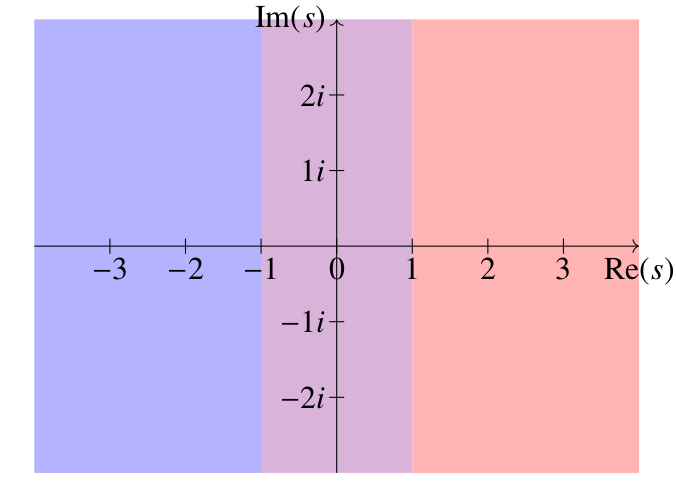
\includegraphics[width=\columnwidth]{graph_1}
\caption{ ROC of $X_1(s)$ and $X_2(s)$  }
\label{graph:ee25-ag3}
\end{figure}

Based on the regions of convergence of  $X_1(s)$ and $X_2(s)$ , we can conclude that option 4) is correct .  





\end{document}
